\documentclass[12pt,a4paper]{article}
\usepackage[margin=3cm, left=4cm, top=2cm, bottom=2cm]{geometry}
\usepackage{graphicx}
\usepackage{subfigure}

\title{\textbf{Synopsis}}

\author{Rahul Bali\\16205025\\Department of Computer Science and Engineering\\Punjab Engineering College, Chandigarh}


\date{\today}

\begin{document}
	\maketitle

	\section{Introduction}
	During the last decade, the importance of recommender systems has been increasing to the point that the success of many well-known service providers depends on these technologies. Recommender systems can assist people in their decision making process by anticipating preferences. However, common recommender algorithms often suffer from lack of explicit feedback and the “cold start” problem. This thesis investigates an approach of using implicit data only, to extract users’ intent for fashion e-commerce in cold start situations. Markov Decision Processes (MDPs) are used on web session data to extract topic models. This thesis also explores how well the topic models can capture users intent and whether they can be used to produce good recommendations. The results show that this approach was able to accurately identify sessions topics, and in most cases the topics could successfully be translated to product recommendations.\\

	Recommender systems have become the most popularly unpopular area in the field of machine learning. It is being used widely yet it is behind the noticeable frame of people's vision. Recommender systems have been the major milestones in the application of Computer Science to other areas. This can be categorized into collaborative-filtering, content based RS and some Hybrid Approaches.\\
	
	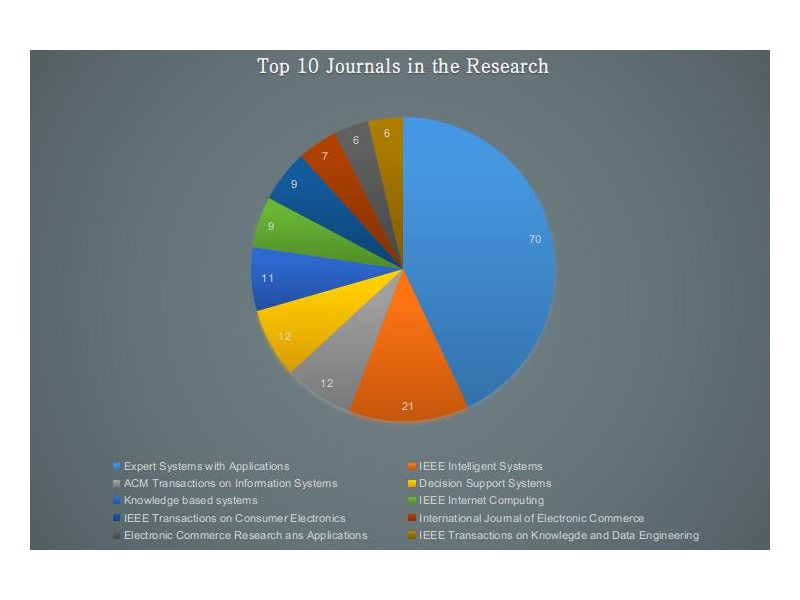
\includegraphics[width=\linewidth]{images/Untitled1.png}\\

Content-based RS focuses on building user profile of a single user for recommendations while collaborative-filtering(CF) RS uses data from fellow users/peers to recommend a particular user. Content-based RS has its roots in Information Retrieval, utility function is defined for each item for a user based on the history of the user purchases, searches, etc. Usually, higher the utility function value, higher is the preference for recommendation. Limited feature Extraction leads to limited possible recommendations. Also, only domain specific recommendations can be inferred. New user problem exists for the both kind of the RS systems. Almost no information is present about the new users into the application environment.\\

Collaborative-filtering techniques create user groups / clusters based on similar tastes / browsing habits, and few techniques consider stereotypes for peer groups. And collaborative-filtering is of two types based on the data mining techniques; heuristics (memory) based, model-based CF. Both techniques have decent application in the industry for real world problem solving. Improvements have been shown in the combined use of these data mining techniques.\\

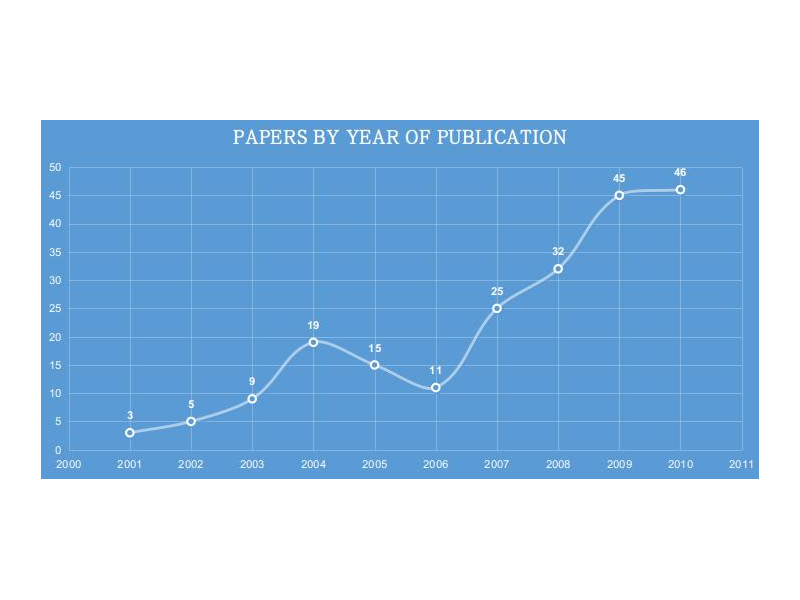
\includegraphics[width=\linewidth]{images/Untitled}\\

In memory-based CF, similarity among users is calculated using cosines of the user matrices. Correlation and similarity are calculated by heuristic techniques.Heuristics basically work by aggregation or summation(∑) of the past activities of the users who are similar to a user for whom recommendations are required. Another is Model-based CF, models are prepared based on ANN, K-means clustering, Gibbs sampling, Probabilistic latent semantic analysis, generative semantics of latent Dirichlet Allocation. CF recommendation systems also faces few issues; new item problem, in which recommendations of this new item are not made to any use because of the shortage of the data. Sparsity, this issue arises for a user whose tastes are fairly diverse from the other users which increases hardness of the recommendations. Demographic-based filtering and preference-based filtering could be helpful with these kind of limitations. Preference-based filtering is currently high on research and industry use.\\

	\newpage
	\section{Literature Review}
	
	\cite{adomavicius2005toward} talks about the field of recommender system from the generation point of view. It classifies recommender systems into three categories: content-based, collaborative, hybrid recommendation approaches. \\
	
	\cite{park2012literature} is reviewing the already existing literature and tries to classify each into recommendation systems research.\\
	
	\cite{linden2003amazon} describes the base use of Recommender system technology in the industry sector of the E-commerce applications.\\
	
	\cite{sarwar2001item} shows how one can define and implement the Recommender systems for the real world application.\\
	
	\cite{konstan1997grouplens} Grouplens Research undertook the task of achieving non-intrusive technology for getting the explicit ratings.\\
	
	\cite{schein2002methods} Metrics are created to measure the effectiveness of the predictions of the results of recommender systems.\\
	
	\cite{tintarev2011designing} user perspective into the recommendation trust they can have, providing explanation for the way recommendations are provided helps user gain trust into the service.\\
	
	\cite{ricci2011introduction} describes the role of recommender systems for the user and the service providers. Providers have got much inclination to recommender systems which has proved to be beneficial for many past decade.\\
	
	\cite{ekstrand2011collaborative} The differing personalities exhibited by different recommender algorithms show that recommendation is not a one-size-fits-all problem. Specific tasks, information needs, and item domains
	represent unique problems for recommenders, and design and evaluation of recommenders needs to be done based on the user tasks to be supported.\\
	
	\newpage
	\section{Problem Formulation}

	\textbf{}	\\Producing high quality recommendations, performing many recommendations per second for millions of users and items and achieving high coverage in the face of data sparsity. In traditional collaborative filtering systems the amount of work increases with the n umber of participants in the system. New recommender system technologies are needed that can quickly produce high quality recommendations, even for very large-scale problems. To address these issues we have explored item-based collaborative filtering techniques. Item-based techniques first analyze the user-item matrix to identify relationships between different items, and then use these relationships to indirectly compute recommendations for users. 

	\section{Objectives}
	\begin{enumerate}
		\item{To review performance of existing algorithms for high quality results in the recommendations.}
		\item{To produce improved performance and novel methods and techniques.}
		\item{Implement the recommender systems in the Python Language.}
		\item{Comparison of the our algorithm and Improved versions.}
	\end{enumerate}
	\textbf{}\\



	
	 
	%\graphicspath{E:\Own\PEC---\ME 3 SEM\recommender-research\images}
	%\textbf{}\\
	
	\newpage
	\bibliographystyle{IEEEtran}
	\bibliography{references}
	



\end{document}

